\section{Lecture 1}

Metric spaces\\
Cayley graphs\\

If a group $G$ is finitely generated, any finite generating $S$ subset defines a metric called the word metric $d_S$. The metric space $(G,d_S)$ is denoted by $|G|_S$. We always suppose the subsets to be symmetric and to not contain the neutral element. Two such metric are always linearly equivalent, and $|G|$ denotes the equivalence class of these metric spaces. To $|G|_S$ is associated a undirected graph, that is a metric one-dimensional complex. The vertex set is the group, $V= G$, whereas two vertices are connected by an edge if $d(s,t)=1$, which means in the word metric that $s^{-1}t\in S$.\\

In the case when $G$ is residually finite with respect to $\mathcal N$, we can build the box space $X_{\mathcal N}$. Here $\mathcal N=\{N_i\}_i$ is a decreasing sequence of finite index normal subgroups of $G$ with rivial intersection. Fix a finite symmetric non-degenerate generating set $S$, and let $S_i$ be the image of $S$ in the finite quotient $G_i= G/N_i$. The box space is defined as the coarse disjoint union of the $|G_i|_{S_i}$,
\[X_{\mathcal N} = \coprod_i |G_i|_{S_i}. \] 

Ref: chapter 1 of Nowak, Yu, Large Scale geometry.
\section{Lecture 2}

What kind of morphisms should we use between metric spaces? We would like to find maps that capture the large scale geometric information between spaces.\\

We already have seen that isometries, i.e. maps $f : X\rightarrow Y$ such that $d(f(x),f(y)) = d(x,y)$ are too rigid. For instance, we would like to say that two Cayley graphs of the same finitely generated group look the same from far away. 

\begin{definition}
A quasi-isometry between metric spaces is a map $f : X\rightarrow Y$ such that there exist $L,C>0$ satisfying
\[\frac{1}{L} d(x,y) - C \leq d(f(x),f(y)) \leq L d(x,y) + C \quad \forall x,y \in X,\]
and there exists $r>0$ such that 
\[Y = \cup_{x\in X} B(f(x), r).\]
\end{definition}

Example: $(G,d_S)$ and $(G,d_T)$ are quasi-isometric. (Proof in class)\\

An action of a discrete group $G$ on $X$ is properly discontinuous if for every compact subset $K\subset X$
\[ | \{ g\in G  \ : \ gK \cap K \neq \emptyset \} | <\infty.\]

\begin{thm}
Let $X$ be a proper geodesic space, and $G$ a discrete group acting on $X$ by isometries. If the action is properly discontinuous and cocompact then $G$ is finitely generated and is quasi-isometric to $X$.
\end{thm} 

$S = \{ g \ : \ B(x_0, r)\cap B(gx_0,r)\neq \emptyset \}$.

Applications: 
\begin{itemize}
\item[$\bullet$] if $M$ is a compact Riemannian manifold and $G=\pi_1(M)$, then $G$ and the universal cover of $M$ are quasi-isometric (with the lifted $G$-invariant metric)
\item[$\bullet$] $PSL(2, \Z)$ is quasi-isometric to the upper-half plane with the hyperbolic metric $\frac{dx^2+dy^2}{y}$, hence to $\mathbb F_2$. The first point gives the generators.\\
\end{itemize}

Coarse maps and coarse embedding: definitions.\\

\begin{prop}
Any metric space admits an isometric embedding into a Banach space.
\end{prop}

$\phi(x) : X\rightarrow l^\infty (X) ;  s \mapsto d(s,x) - d(s,x_0)$.\\

We will be interested in the following question: when does a space a coarse embedding into a real Hilbert space?\\

Some examples of Hilbert spaces: $l^2(X)$, $l^2(X,H)$, $L^2(\Omega, \mu)$, random variable with second moments with $E(XY)$.\\

Definition of Hilbert spaces\\

A remark: the inner product can have a non-trivial null-space, Cauchy Schwartz still holds. In particular, the null-space will be a subspace and inner product is definite on the quotient. The \textit{separation-completion} of a real vector space $V$ will be 
\[H = \overline{V /N }^{\| .\|}.\]
It is a real Hilbert space.\\
 
Example: we have seen that $\Z^n$ is quasi-isometric to $\R^n$ with the Manhatthan metric, itself quasi-isometric to the Euclidean metric so $Z^n$ is CEH. Indeed
\[\sum_{i=1}^n |x_i | = \langle x,\epsilon\rangle \leq \| x\|_2 \|\epsilon \|_2 = \sqrt{n} \| x\|_2 .\]
Also: trees are CEH, $l^1(\mathbb N)$ is CEH. (Proofs)\\

Definition: positive definite kernels.\\

Example: Let $\phi: X\rightarrow H$ be any map. Then $k(x,y) = \langle \phi(x) , \phi(y)\rangle $ is a pdk.

\begin{thm}
Let $k: X\times X \rightarrow \R$ be a positive definite kernel. Then there exists a real Hilbert space and a map $\phi: X \rightarrow H$ such that 
\[k(x,y) = \langle \phi(x) , \phi(y)\rangle  \quad \forall x,y \in X.\]
\end{thm}

\begin{proof}
Let $V$ be the linear space of finitely supported real functions on $X$. Define
\[ \langle f , g \rangle = \sum_{x,y} f(x)f(y) k(x,y) \quad \forall x,y\in X.\]
It might happen than this inner-product has a nullspace. Let $H$ be the separation-completion of $V$.
Define \[\phi : X\rightarrow H ; x \mapsto e_x\]
where $e_x(x') = 1_{x=x'}$. Then
\[ \langle \phi(x) , \phi(y)\rangle = \sum_{x,y} e_x(x')e_y(y') k(x',y') = k(x,y). \] 
\end{proof}

Ref: Chapter 1 and 5 of Nowak, Yu, Large scale geometry.

\section{Lecture 3}

Last time we defined coarse embeddings and quasi-isometries. An interesting example of a coarse embedding that may not be a quasi isometriy is the inclusion of a subgroup $H$ into a group $G$.

To see that, consider the Baumslag Solitar group 
\[G =BS(1,2) = \langle a, b \  : b^{-1}ab = a^2 \rangle ,\]
and let $H = \langle a \rangle \cong \Z$. One sees that, whereas $l_H(a^n) = n$, the relation $a^{2^n} = b^{-n}a b^n$ ensures that $l_G(a^{2^n}) \leq 2n+ 1$, so that $l(a^n)$ is of the same order as $log_2(n)$. 

\subsection{Kernels}

A symmetric kernel on $X$ is a function $k: X\times X \rightarrow \R $ such that $k(x,y) = k(y,x)$. It is
\begin{itemize}
\item[$\bullet$] of positive type if for every finite subsets $F \subset X$
\[\langle v , K_F v \rangle \geq 0 \quad \forall v \in l^2(F).\] 
\item[$\bullet$] of conditionally negative type if for every finite subsets $F \subset X$
\[\langle v , K_F v \rangle \leq 0 \quad \forall v \in l^2(F)\text{ s.t. }\sum_{x\in F} v_x = 0.\] 
\end{itemize}

Examples: constants are (PT) and (CNT), for any map $f : X\rightarrow \R$, $k(x,y) =f(x)f(y)$ is (PT). If $k$ is (PT), $-k$ is (CNT). It is the conditionally that is here important, otherwise, it would be the opposite of being positive.\\

Operations on kernels: (PT) and (CNT) both form a cone (stability by addition and multiplication by a positive scalar), they are closed for the topology of simple convergence and by Schur multiplication. \\

Pb: show that Schur multiplication preserves (PT).\\

\begin{prop}
Let $k: X\times X\rightarrow \R $ be a positive type function on $X$ and $f(x)=\sum_n a_n z^n$ an entire function with positive coefficients. Then
\[\sum_n a_n k(x,y)^n\]
defines a positive type function. 
\end{prop}

\begin{thm} Schoenberg's lemma. Let $k: X\times X\rightarrow \R $ be a symmetric kernel on $X$. Then $k$ is (CNT) iff 
\[\forall t> 0 , \exp (-tk(x,y))\]
is of positive type.
\end{thm}

\begin{proof}
If $e^{-tk(x,y)}$ is (PT) for every $t>0$, then 
\[k(x,y) =\lim_{t\rightarrow 0} \frac{1-e^{-tk(x,y)}}{t}\]
is (CNT).\\

If $k(x,y)$ is (CNT), then there exists a real Hilbert space $H$ and a map $\phi: X \rightarrow H$ such that 
\[k(x,y) = \| \phi(x) - \phi(y) \|^2 \quad \forall x,y \in X.\]
Then
\[e^{-tk(x,y)} = e^{-t \| \phi(x) \|^2 } e^{-t \| \phi(y) \|^2 } e^{2t \langle \phi(x), \phi(y) \rangle } \]
is a Schur product of a kernel of the type $f(x)f(y)$ with the exponential of a positive type, so it is positive. 
\end{proof}

Remark on the GNS construction.

When $k(x,y)$ is (CNT) then the separation completion of 
\[V = \{a : X\rightarrow \R \text{ finitely supported s.t. }\ : \ \sum_x a_x = 0\}\]
with respect to the positive bilinear form 
\[\langle a, b \rangle = -\frac{1}{2}\sum_{x,y} a_x b_x k(x,y) \]
gives a real Hilbert space $H$ and map $\phi: X \rightarrow H$ such that 
\[k(x,y) = \| \phi(x)-\phi(y) \|^2 \]
and $span\{\phi(x) - \phi(x_0)\}_{x\in X} $ is dense in $H$, where $x_0$ is any fixed point.\\ 

The couple $(H, \phi)$ is unique up to affine isomorphism: if $(K, \Psi)$ is another such couple, there exists a unique affine isomorphism $A: H \rightarrow K$ such that $\Psi =A\circ \phi $. 
 
\subsection{Kernels and approximation properties}

A function $\eta: X\times X \rightarrow \R$ is
\begin{itemize}
\item[$\bullet$] proper if $\eta^{-1}([-r,r])$ is an entourage for every $r>0$,
\item[$\bullet$] $\sup_{(x,y)\in \Delta_R} | \eta(x,y) | < \infty$.
\end{itemize}

\begin{thm}
Let $X$ be a countable discrete space with bounded geometry. Then the following are equivalent:
\begin{itemize}
\item[$\bullet$] X admits a coarse embedding into Hilbert space
\item[$\bullet$] there exists a proper \text{conditionally negative} type function that is bounded on entourages.
\end{itemize}
\end{thm}

First implication: $\eta(x,y) = \| \phi(x) - \phi(y)\|^2$.\\

Definitions: $G$ residually finite w.r.t. $\mathcal N = \{N_n\}$, $q_n: G \rightarrow G_n = G/N_n$, box space
\[X_{\mathcal N} = \coprod Cay(G_n, q_n(S)).\]
Haagerup's property or a-T-menability.

\begin{prop}
If $X_{\mathcal N}$ is (CEH), then $G$ is a-T-menable.
\end{prop}

\begin{proof}
By definition, we get a sequence of negative type functions 
\[\phi_n : G_n \rightarrow H\]
with 
\[\rho_-(l_n(x)) \leq \phi_n(x) \leq \rho_+(l_n(g)).\]
The composition $\phi_n\circ q_n$
\end{proof}

Remark: the converse does not hold: the free group on $n$ generators is a-T-menable, and any finitely generated group is a quotient of a $\mathbb F_n$, so we get a coarse embedding
\[X(G) \rightarrow X(\mathbb F_n)\]
so that the converse to the last proposition would imply that any box space is (CEH). But any infinite residually finite property (T) group contradicts this, $SL(3,\Z)$ for instance.\\

Ref: Chapter 5 and 6 of Nowak, Yu, Large scale geometry, and Appendix C of Bekka, Valette, Kazdhan Property (T)

\section{Lecture 4}

Definition of the Laplacian on a graph: for any Hilbert space $H$,
\[(\Delta f)(x) = f(x) - \frac{1}{N_x}\sum_{y : (x,y)\in E} f(y)\quad \forall f\in l^2(X,H).\]
On a finite graph, the Laplacian is a symmetric (or selfadjoint in the complex case) positive matrix with kernel the constant functions, and its orthogonal is 
\[ker(\Delta)^\perp = \{ f\in l^2(X) \ : \ \sum_{x\in X} f(x) = 0\}.\]

\subsection{Expanders}

\begin{definition}
An expander sequence is a sequence of finite graphs $X_n= (V_n, E_n)$ such that 
\begin{itemize}
\item[$\bullet$] $\lim_n |V_n| = +\infty $,
\item[$\bullet$] $d=\sup_n deg(X_n)< \infty$,
\item[$\bullet$] there exists a constant $c>0$ such that, for every $n$, $sp(\Delta_{X_n}) \subset \{0\} \cup (c,\infty)$.
\end{itemize}
\end{definition} 

Out of an expander sequence, we build its \textit{coarse disjoint union}
\[X = \coprod X_n\]
which is the disjoint union as a set, endowed with a metric $d$ which restricts to the graph metric on any of the graphs, and such that $\lim_{i,j\rightarrow \infty} d(X_i,X_j)=+\infty$. It is $X$ that we call an expander.\\

The last condition means that for every $f\in l^2(X,H)$ such that $\sum_{x\in X_n} f(x)=0$, the inequality
\[\sum_{(x,y)\in E_n} \| f(x)-f(y) \|^2 \geq c \sum_{x\in X_n} \| f(x)\|^2    \]
holds.

\begin{thm}
Expanders cannot admit a coarse embedding into Hilbert space.
\end{thm}

\begin{proof} 
I think this proof is due to Higson. Let $f: X \rightarrow H$ be a coarse embedding. One gets vectors $f_n\in l^2(X_n,H)$ by restricting $f$ to $X_n$. We can translate each $f_n$ without changing the fact that it is a coarse embedding, so we can suppose $\sum_{x\in X_n} f_n(x)=0$, hence
\[\sum_{(x,y)\in E_n} \| f_n(x)-f_n(y) \|^2 \geq c \sum_{x\in X_n} \| f(x_n)\|^2.\]
The term on the left is less than $d |V_n| \rho_+^2(1)$ so that we get a inequality of the type
\[\sum_{x\in X_n} \| f(x_n)\|^2 \leq A |V_n|\]
with $A$ a constant independent of $n$. That is possible only if at least half of the terms are less than $2A$. But that is a contradiction with the properness of $f$, since it means that $f_n$ maps more than $\frac{|X_n|}{2}$ terms into $B(0,2A)$.\\	 
\end{proof}

We will understand better the following diagram
\[\begin{tikzcd}
\text{amenablity} \arrow{r}\arrow{d} & \text{a-T-menability} \arrow{d} \\
\text{ property (A)} \arrow{r} & \text{ (CEH) }  
\end{tikzcd}\]
where the top row is a $G$-equivariant version of the bottom one, whereas the left side corresponds to finitely supported kernels, relaxed into a $c_0$ condition on the right. There is a parallel diagram with property (T), and we will see what should be a non-equivariant version of property (T). There is a way to restore equivariance by considering the \textit{coarse groupoid}.

\subsection{GNS construction}

We have seen that for any symmetric kernel $k: X\times X \rightarrow \R$ of positive type, there exists a pair $GNS(k)=(H,\phi)$ satisfying
\begin{itemize}
\item[$\bullet$] $H$ is a real Hilbert space,
\item[$\bullet$] $\phi : X\rightarrow H$ is a map such that $\langle \phi(x),\phi(y) \rangle = k(x,y)$ and $span \{ \phi(x)\ : \ x\in X \} $ is dense in $H$. 
\end{itemize}

Moreover, the pair $(H,\phi)$ satisfies the following universal property: let $(K,\psi)$ be any other pair such that $\langle \psi(x),\psi(y) \rangle = k(x,y)$. Then there exists a unique linear isometry $T: H\rightarrow K$ such that $\psi = T \circ \phi$.\\

Indeed, the identity 
\[\langle \sum_i a_i \delta_{x_i}, \sum_j b_j \delta_{y_j} \rangle  = \sum_{i,j} a_i b_j k(x_i,_j) =\langle \sum_i a_i \psi(x_i), \sum_j b_j \psi(y_j) \rangle\]
proves that the map $\sum_i a_i \delta_{x_i}\mapsto  \sum_i a_i \psi(x_i)$ extends to an isometry $T:H \rightarrow K $ satisfying $\psi = T \circ \phi$. Uniqueness is obvious.\\

Now, say that $X=G$ is a group, and that the kernel is $G$-equivariant, i.e.
\[k(gx,gy) = k(x,y)\quad \forall g,x,y\in G.\]
Such a function is entirely determined by 
\[\tilde k (g) = k(e,g),\]
which is then what is called a positive type function on the group $G$.\\

In this case, the GNS construction and its universal property allows to build a unitary representation. Indeed 
\[\langle \phi(gx),\phi(gy) \rangle = k(gx,gy) = k(x,y)\] 
ensures the existence of a unique linear isometry $\pi_g: H \rightarrow H$ such that $\phi(gx) = \pi_g \phi(x)$, $\forall g,x \in G$. The uniqueness also ensures that $\pi_s \pi_t = \pi_{st} $ and $\pi_e = id_H$. Together with symmetry ($\tilde k(g^{-1})=\tilde k(g)$), it implies that $\pi_g^*=\pi_{g^{-1}}$. So that, if $v= \phi(e)\in H$, we have that the GNS pair $(H,\phi)$ is actually equivalent to a triple $(H,\pi, v)$ where 
\begin{itemize}
\item[$\bullet$] $H$ is a real Hilbert space,
\item[$\bullet$] $\pi : G\rightarrow U(H)$ is a unitary representation, 
\item[$\bullet$] $v\in H$ is a vector,
\end{itemize}
such that $span \{ \pi_g (v)\}_{g\in G}$ is dense in $H$ (we say $v$ is \textit{cyclic} for $\pi$), and $\tilde k(g)=\langle v , \pi_g (v)\rangle$, for all $g\in G$.\\

The triple $(H,\pi,v)$ is called the GNS triple associated to the positive type function $\tilde k$. It satisfies the following universal property: if $(K,\sigma , w)$ is any other triple such that $\tilde k(g)=\langle w , \sigma_g (w)\rangle$, then there exists a unique linear isometry $T: H\rightarrow K $ such that $Tv= w$ and $T\pi_g = \sigma_g T$.\\

As a problem, show that the GNS triple of a cyclic representation is unitarily equivalent to the original representation, i.e. 
\[GNS(\pi_{v,v}) \cong (H,\pi,v).\]  

As a result, we get that the family of equivalence classes of cyclic representation is a set, isomorphic to the set of positive type functions on $G$.
\[\{ \pi: G\rightarrow U(H) \text{ cyclic } \} / \sim \cong \{\phi : G \rightarrow \R \text{ positive type}\}.\] 

We will see next time how we can use a natural topology on the space of bounded functions on $G$ to topologize the space of cyclic representations of $G$. (This will be equivalent to the Fell topology)

\section{Lecture 5}
Recall that cyclic unitary representations corresponds to positive type functions on the group via the GNS construction. Cauchy-Schwartz ensures that
\[|\phi(g) | = |\langle v_\phi , \pi_\phi(g)v_\phi \rangle | \leq \|v_\phi \|^2,\]
hence $\phi\in l^\infty(G)$, and $\|\phi\|_\infty = |\phi(e)| =\|v_\phi \|^2$. But $(l^\infty(G), \|\cdot\|_\infty )$ is a Banach space. 
\[\tilde G\cong \mathcal C :=\{\phi: G\rightarrow \R \text{ PT s.t. }\phi(e) = 1\}\] 
Positive type functions form a cone closed w.r.t the topology of pointwise convergence, so the weak-$*$ topology. $\mathcal C$ is a closed convex subspace, so that Krein-Milman ensures that the set of extremal points is weak-$*$ dense in $\mathcal C$.

\begin{prop}
$Ext(\mathcal C)$ corresponds to the irreducible unitary representations via the GNS-construction.
\end{prop}  
 
This is an easy consequence of how the operations on positive type functions tranlate at the level of representations.
\[GNS(t\phi)\cong (H_\phi, \pi_\phi, \sqrt{t}\cdot v_\phi)\]
\[GNS(\phi_1+\phi_2)\cong (H_{\phi_1} \oplus H_{\phi_2}, \pi_{\phi_1}\oplus \pi_{\phi_2}, v_{\phi_1}\oplus v_{\phi_2})\]
\[GNS(t\phi)\cong (H_{\phi_1} \otimes H_{\phi_2}, \pi_{\phi_1}\otimes \pi_{\phi_2}, v_{\phi_1}\otimes v_{\phi_2})\]

The set of equivalence classes of unitary representations is endowed with the Fell topology: it is the topology of uniform convergence of coefficients on compact subsets. It corresponds exactly to the weak-$*$ toplogy on the space of normalized positive type functions.

\begin{thm} [Raikov]
The weak-$*$ topology and the topology of uniform convergence on compact subsets, i.e. for every net $\phi_i$ of positive type normalized functions 
\[ \forall f \in l^1(G), \quad \lim_i\langle \phi_i , f\rangle = \langle \phi , f\rangle \iff \forall F\subset G\text{ finite}, \quad \lim_i\|\phi_i -\phi\|_{\infty , F} = 0 \] 
\end{thm} 
\begin{proof}
Let $\phi_i$ converge uniformly on every finite subsets to $\phi$. Let $f\in l^1(G)$ and $\varepsilon>0$. There exists a finite subset $F\subset G$ such that 
\[\sum_{g\in G-F} |f(g)| \leq \frac{\varepsilon}{4}\]
and a rank $n$ such that 
\[\forall i\geq n, \|\phi_i -\phi\|_{\infty , F} \leq \frac{\varepsilon }{2\sum_{F} |f(g)| }\]
and 
\[\begin{split}
|\langle \phi - \phi_i , f \rangle | & \leq \|\phi_i -\phi\|_{\infty , F} \sum_{F} |f(g)|+2\sum_{G-F}|f(g)| \\
				& \leq \varepsilon \\ 
\end{split}\]
So that $\phi_i$ converges to $\phi$ in the weak-$*$ topology.\\
 
Let $\phi_i$ converge to $\phi$ in the weak-$*$ topology. Let $F\subset G$ be finite, and $\varepsilon>0$. Define $f=\chi_F\in l^1(G)$ and, up to changing the value of $f$ to $-1$, we get that, ultimately,  
\[ |\phi(g)-\phi_i(g)|\leq \sum_{g\in F} |\phi(g)-\phi_i(g)| = \langle \phi - \phi_i , f \rangle   \leq \varepsilon \quad \forall g\in F\]
which ensures that $\|\phi_i-\phi\|_{\infty, F}\leq \varepsilon$.
\end{proof}

Problem: Show that unireps separate points, i.e. for any $s\neq t$ in $G$, there exists a unirep $\pi$ such that $\pi(s)\neq \pi(t)$. \\

Going back to a-T-menability.

\begin{definition} We say that $G$ is a-T-menable, or has Haagerup's property, if there exists a (metrically) proper action of $G$ on a real Hilbert space by affine isometries, i.e there exists a group morphism 
\[\alpha:\left\{\begin{array}{rcl} G & \rightarrow & Aff(H) \\ v & \mapsto & \alpha_g(v) = \pi_g(v)+b_g\end{array}\right.\] 
with 
\begin{itemize}
\item[$\bullet$] $\pi: G \rightarrow U(H)$ is a unitary representation for $G$,
\item[$\bullet$] $b: G\rightarrow H$ is a cocycle for $\pi$, meaning $b_{st} = \pi_s b_t+ b_s$, for every $s,t \in G$,
\item[$\bullet$] $\alpha$ metrically proper, i.e. $\lim_{l(g)\rightarrow \infty} \|b_g\|^2 =\infty$.
\end{itemize}
\end{definition}
Remarks:
\begin{itemize}
\item[$\bullet$] the cocycle relation ensures that $\alpha $ is a group morphism. In particular, it also yields 
\[ \|b_s- b_t\|^2 = \| b_{s^{-1}t} \|^2 ,\]
ensuring that $\phi(g)=\|b_g- b_e\|^2$ is a conditionally negative type function on $G$.
\item[$\bullet$] 
\end{itemize}

\begin{thm} If $G$ is a-T-menable, then $G$ admits a coarse embedding into Hilbert space.
\end{thm}
\begin{proof}
It suffices to show that $\phi(g)=\|b_g- b_e\|^2$ is proper, which is guaranted by the fact that $\lim_{l(g)\rightarrow \infty} \|b_g\|^2 =\infty$.\\
\end{proof}

An interesting consequence is the following. 
\begin{prop}
If $G$ is a-T-menable, there exists a continuous path of representations between the trivial representation and the quasi-regular representation $\lambda_{G/H}$ for some subgroup $H<G$.
\end{prop}

\begin{proof} By Schoenberg's lemma, for every $t>0$, 
\[\phi_t(g) = \exp(-t\eta(g))\]
is of positive type. Let $\Psi$ be the characteristic function of $\{ g\ : \ \eta(g) = 0\}$. Let s show that $\phi_t$ converges uniformly on finite subsets to $\Psi$ as $t$ diverges to infinity. Let $F\subset G$ be finite, then its obvious isn't it?\\

Claim: $H= \{ g\ : \ \eta(g) = 0\}$ is a subgroup of $G$. Indeed $\eta(e)=0$ and 
\[\eta(s^{-1}t) \leq (\eta(s)+\eta(t))^2. \]

\[\|a\|^2_\Psi = \sum_{x\in G/H} (\sum_{s\in xH} a_s)^2\]
so that $N = \{a \ : \ \forall x\in G, \sum_{s\in xH} a_s = 0\}$ and
\[V/N \cong span \{ \chi_{xH}\}_{x\in G} \]
hence $H_{\Psi}\cong l^2(G/H)$ and $\pi_\Psi(g)\chi_{xH}= \chi_{gxH}$, $v_\Psi = \chi_{H}$, so that $GNS(\Psi)$ is isomorphic to the quasi-regular representation on $G/H$.\\	

This gives $GNS(\phi_t)$ converges in the Fell's topology to $\lambda_{G/H}$.
\end{proof} 

References: Bekka, Valette, Property T (Annex C)\\
Nowak Yu, Chapter on isometric actins on Banach spaces\\

\section{Lecture 6}

A last remark on affine actions of groups by isometries on Hilbert spaces. In the same way that a positive type kernel is equivalent to a Hilbert space $H$ and a map $\phi : X \rightarrow H$, there is an algebraic relation for cocyles: a cocycle for an isometric representation $G\rightarrow Aff(H)$ is equivalent to a negative type function $G\rightarrow \R$. Indeed, given such a cocycle $b: G \rightarrow H$,
\[\phi(s^{-1}t) = \|b_s-b_t\|^2=\| b_{s^{-1}t}\|^2\]
defines a negative type function, and the GNS representation associated to a CNT on $G$ will give a cocyle. Moreover, if the group is of bounded geometry, there is automatically a nondecreasing function $\rho_+$ such that $\|b_s-b_t\|\leq \rho_+(d(s,t))$, since 
\[\phi(g) \leq \sup_{x\in B(e,r)} \phi(x) \quad \forall g : |g|\leq r, \]
because the balls are finite. The only missing condition for $b$ to be a coarse embedding is the bound on the left hand side, which is equivalent to being proper. Notice that the opposite of a proper cocycle is any so called coboundary 
\[b_g = v-\pi_g(v)\]
which is bounded. In that case, $\alpha_g(v)=v$ is a constant representation.\\

Then: discussion on the origin of amenability, i.e. the Banach Tarski paradox. Vitali's theorem: there exists measure define on the whole of $P(\R)$ such that $\mu([0,1]) = 1$ and which is $\sigma$-additive and invariant by translation, whence the need to introduce $\sigma$-algebras. In the other way, we can define finitely additive measures, which we can show to be equivalent to means.\\

Let $X$ be a metric space, possibly endowed with an isometric action of $G$.

\begin{definition}
A mean on $X$ is a normalized ($m(1_X)=1$) positive ($m(f)\geq 0$ when $f\geq 0$) linear functional $m: l^\infty(X)\rightarrow \C$. We say that $m$ is $G$-invariant if 
\[m(\alpha_g(f))=m(f) \quad \forall f\in l^\infty (X), g\in G.\] 
\end{definition}

A mean is automatically continuous of norm $1$, and is thus an element of the dual $l^\infty(X)^*$. The space of means is a convex that is compact for the weak-$*$ topology.

\begin{definition}
A group $G$ is amenable if any of these equivalent conditions are satisfied:
\begin{itemize}
\item[$\bullet$] there exists a $G$-invariant mean on $l^\infty(G)$,
\item[$\bullet$] there exists a finitely additive measure on $G$, invariant by $G$-translation, 
\item[$\bullet$] for all $\varepsilon>0, r>0$, there exists a finite subset $F \subset G$ such that 
\[ \forall |g|\leq r, \frac{|F\Delta gF|}{|F|}< \varepsilon\]
\item[$\bullet$] for all $\varepsilon>0, r>0$, there exists a finite subset $F \subset G$ such that
\[\frac{|\partial_r F|}{|F|}<\varepsilon\]
\end{itemize}
\end{definition}

The definition via means is powerful to show that the following are amenable.
\begin{itemize}
\item[$\bullet$] finite groups
\[m(f)=\frac{1}{|G|}\sum_{g\in G} f(g),\]
\item[$\bullet$] if $G$ is amenable, so is $G/N$ where $N$ is a normal subgroup. Define a map $l^{\infty}(G/N)\rightarrow l^\infty(G)$ by identifying functions on $G/N$ to functions on $G$ that are constant on cosets,
\item[$\bullet$] abelian groups. Dualize the action of $G$ on $l^\infty(G)$ to the convex compact $K$ of means on $G$: we get affine maps $\tilde \alpha_g : K\rightarrow K$ for each $K$. By Kakutani's theor	em, they each have at least a fixed point. Since the affine maps commutes, the fixed points are stabilized so that for every finite subset $F\subset G$,
\[\cap_F Fix(\tilde \alpha_g)\]
is nonempty. Baire's theorem ensures that $\cap_G Fix(\tilde \alpha_g)$ is non-empty, so there exists a $G$-invariant mean.
\end{itemize} 

The implication from definition by Folner sets to the one by mean also uses a compactness argument: for any Folner set, define 
\[m_F(f)= \frac{1}{|F|}\sum_{g\in F}f(g).\]
Then $\{m_F\}$ is a bounded net in $K$ so that there exists an accumulation point which is easily shown to be an invariant mean.\\

For extensions, amenability satifises the ``2 out of 3'' property. This implies, knowing that abelian groups are amenable, that solvable groups are amenable.\\

The free group is not amenable. If a group is not amenable, then there is a constant $C>0$ such that 
\[\frac{|\partial_r F|}{|F|}\geq C\]
for every finite subset $F\subset G$. In particular
\[|B(e,n)| = \prod_{k=1,n} (1 + \frac{|S(e,k)|}{|B(e,k)|}) \geq (1+C)^n.\]
 In particular, subexponential growth implies amenability. So $\Z^n$ is amenable (not using that it is abelian).
 
Next time:
Hulancki-Reiter conidition for amenability, Property A and Higson-Roe condition (analog of Reiter), and kernel characterization 
\begin{thm}
X has property (A) iff for every $r>0, \varepsilon>0$, there exist $s>0$ and a positive type kernel $\phi: X\times X\rightarrow \R$ such that 
\begin{itemize}
\item[$\bullet$] $supp \ \phi \subset \Delta_s$,
\item[$\bullet$] if $d(x,y)\leq r$, $|1-\phi(x,y)|<\varepsilon$.
\end{itemize}
\end{thm}
Version for amenability: equivariance.\\

Then: formulation in terms of Schur multipliers.

References: Choimet, Queff\'elec, Analyse math\'ematiques, les grands th\'eor\`emes du XXe si\`ecle.\\
Nowak Yu, Chapter on amenability\\

\section{Lecture 7}

Let us prove that amenability implies a-T-menability. For this we will use yet another characterization of amenablity, called the Hulanicki-Reiter condition.

\begin{thm}
$G$ is amenable iff for all $r>0,\varepsilon >0$, there exists a finitely supported function $f\in l^1(G)_{+,1}$ such that 
\[ \| f -s\cdot f\|_1 \leq \varepsilon \quad \forall |s|\leq r. \]
\end{thm}
\begin{proof}
If $G$ is amenable, let $F$ be a $(\varepsilon, r)$-Folner set. The function $f=\frac{1}{|F|}\chi_F$ satisfies the condition\\

Let $f\in l^1(G)_{+,1}$ be as above. Up to a minor approximation, we can suppose $f$ is a step function with rational values: $f(x)\in \{0, \frac{1}{N}, ... , \frac{N-1}{N}, 1\}$. Define
\[F = \{ (g,i) \ : \ i\leq f(g)\} \subset G\times \mathbb N,\]
which is a grid under the graph of $f$, so that, as $f$ is a step function, 
\[1 = \| f \|_1 = \frac{|F|}{N}\]
and if $|s|\leq r$,
\[\frac{|F\Delta sF|}{N} = \frac{|F\Delta sF|}{|F|}= \|f- s\cdot f\|_1 \leq \varepsilon\]
so that $F$ is a $(\varepsilon, r)$-Folner set.
\end{proof}

Remark: we could have taken $f$ in $l^2(G)_{+,1}$. (Problem)

\begin{cor}
If $G$ is amenable, $G$ is a-T-menable.
\end{cor}

\begin{proof}
For each $n$, choose $f_n\in l^2(G)_{+,1}$ a $(2^{-n},n)$-Hulanicki-Reiter function:
\[\|f_n-s\cdot f_n\|_2 \leq \frac{1}{2^n} \quad \forall |s|\leq n.\]
Define $\pi_g = \oplus \lambda_g$ the $l^2$-sum of the left regular representation on $\bigoplus_n l^2(G)$, and 
\[b_g = \oplus_n (f_n - \lambda_g(f_n)).\]
Then 
\begin{itemize}
\item[$\bullet$] $b_g$ is well defined in $l^2$,
\[ \|b_g\|^2 = \sum_n \|f_n - g\cdot f_n\|^2 \leq \sum_{n= 1}^{|g|}\|f_n - g\cdot f_n\|^2 + \sum_{n\geq |g|+1} \frac{1}{4^n}. \]
\item[$\bullet$] $b_g$ is a cocyle for $\pi_g$ (direct computation),
\item[$\bullet$] $b_g$ is proper. Indeed for any $n$, there is a $N_n$ such that $\|f_n -s\cdot f_n\|^2 = 2$ if $|s|\geq N_n$. We can suppose $N_n$ to be increasing, and 
\[\|b_g\|^2 \geq 2|\{n \ : \ N_n \leq |g|\}| \rightarrow +\infty.\]
\end{itemize}
\end{proof}

In his 2000 paper in Inventiones Mathematicae, Guoliang Yu introduced the follwing property.

\begin{definition}
$X$ has property (A) iff for every positive numbers $\varepsilon, r >0$, there exist $s>0$ and a family of finite subsets $\{A_x\}_{x\in X}$ such that 
\[\frac{|A_x \Delta A_y|}{|A_x\cap A_y|} \leq \varepsilon \quad \forall d(x,y)\leq r\]
and $A_x\subset B(x,s)\times \mathbb N$.
\end{definition}

Show that property (A) is a coarse invariant.

Examples:
\begin{itemize}
\item[$\bullet$] finite groups,
\item[$\bullet$] amenable groups,
\item[$\bullet$] trees.
\end{itemize}

In particular, $\mathbb F_n$ is a tree, so it has property (A), while it is not amenable.

We have a analog of the Hulanicki-Reiter condition, called the Higson-Roe condition.

\begin{thm} 
$X$ has property (A) iff for every $r,\varepsilon>0$, there exist $s>0$ and $f:X\rightarrow l^1(X)_{+,1}$ such that 
\[\|f(x)-f(y)\|_1 \leq \varepsilon \quad \forall d(x,y)\leq r\]
and $\text{supp }f\subset B(x,s)$.
\end{thm}

\begin{proof}
If $\{A_x\}$ is a family of subset as in the definition of property (A), then, if $A_x(y) = A_x \cap \{y\}\times \mathbb N$, then 
\[f(x) = \frac{1}{|A_x|}\sum_y |A_x(y)|\delta_y \in l^1(X)_{+,1}\]
satisfies the conditions.\\

If $f: X\rightarrow l^1(X)_{+,1}$ as above is given, then, as for amenability, suppose that $f$ is a step function and define 
\[A_x = \{(x,i)\ : \ i\leq f(x)\}\subset supp(f)\times \mathbb N \subset B(x,s)\times \mathbb N.\]
Then $1 = \|f(x)\|_1= \frac{|A_x|}{N}$, and 
\[\frac{|A_x\Delta A_y|}{|A_x\cap A_y|}\]  

\[ \|f(x)-f(y)\|= \frac{1}{N}\sum ||A_x(z)|-|A_y(z)||  \]  
\end{proof}

References: Nowak-Yu, Chapter on property A

\section{Lecture 8}

We finished the proof of the Higson Roe condition. We use the Higson Roe condition to show the following theorems.

\begin{thm}
If $G$ is an amenable group, it has property (A).
\end{thm}

\begin{proof}
Let $\varepsilon >0, r>0$, and pick a Hulanicki-Reiter function $f\in l^2(G)_{+,1}$, finitely supported and $(\varepsilon, r)$-equivariant. Define $\tilde f (g) = \lambda_{g}^*(f)$. This defines a $(\varepsilon, r)$-Higson-Roe function for $\tilde f : G \rightarrow l^2(G)_{+,1}$.
\end{proof}

\begin{thm}
If $X$ has property (A), it is coarsely embeddable into a Hilbert space.
\end{thm}

\begin{proof}
Let $f_n : X \rightarrow l^2(X)_{+,1}$ be $(\varepsilon_n,r_n)$-Higson-Roe functions for $X$, with $\varepsilon_n = 2^{-n}$ and $r_n = n$. There exists $s_n>0$ such that $supp f_n(x)\subset B(x,s_n)$. We can suppose that $(s_n)_n$ increases and diverges to $+\infty$. Notice that
\[\begin{split}
\sum_n \|f_n(x) - f_n(y)\|^2 & \leq \sum_{n=0}^{d(x,y)} \|f_n(x) - f_n(y)\|^2 +\sum_{n\geq d(x,y)+1} \frac{1}{4^n} \\
				& \leq \sum_{n=0}^{d(x,y)} \|f_n(x) - f_n(y)\|^2 + 2.\\
\end{split}\]
Fix $x_0\in X$. The inequality above says that  
\[F(x) = \bigoplus_n (f_n(x) - f_n(x_0))\]
is well defined as an element of $l^2(X \times \mathbb N)$. It also ensures that
\[ \|F(x)-F(y)\|^2 \leq 2 d(x,y) +2.\]
Moreover, if $d(x,y)> 2s_n$, $\|f_n(x) - f_n(y)\|^2 = 2$, so that 
\[\|F(x)-F(y)\|^2 \geq | \{ n \ : \ 2s_n \leq  d(x,y)\} = \rho_-(d(x,y)),\]
with $\lim \rho_- =\infty$, so that $F$ is a coarse embedding. 
\end{proof}

\subsection{Kernel characterization of property (A)}

Definition of $\C_s[X]$ and $C^*_u(X)$, reminder on how to take the square root of a positive operator in a $C^*$-algebra, via polynomila approximation.

\begin{thm}[Tu]
$X$ has property (A) iff for every $\varepsilon> 0, r>0$, there exists a symmetric normalized positive type kernel $\phi : X\times X \rightarrow \R$ with finite propagation such that $\|1-\phi\|_{\infty, \Delta_r}<\varepsilon$. 
\end{thm}

\begin{proof}
If $X$ has property (A), pick a Higson-Roe function $f: X\rightarrow l^2_{+,1}(X)$ and define $\phi(x,y)=\langle f(y), f(x)\rangle$. It satisfies all the coniditions of the theorem.\\

Let $\varepsilon, r>0$ and $\phi$ be a kernel as above. Let $s= prop(\phi)$. Then
\[(T\xi)(x)= \sum_{y\in X} \phi(x,y)\xi(y) \quad \forall \xi \in l^2(X)\]
defines a bounded operator. Indeed, by the Cauchy-Schwartz inequality
\[\begin{split}
\langle \eta, T\xi \rangle & \leq \sum_{x,y} |\phi(x,y)| |\xi_y| |\eta_x| \\
				& \leq \left( \sum_{x,y}|\phi(x,y)||\xi_y|^2\right)^{\frac{1}{2}}\cdot \left( \sum_{x,y} |\phi(x,y)| |\eta_x|^2 \right)^{\frac{1}{2}}\\
				& \leq N(S) \|\xi \|\|\eta\|
\end{split}\] 
hence $\|T\|\leq N(S)$. Then let $P$ be a polynomial of degre $d$ such that $\|P(T)-T^2\|\leq \varepsilon$, and define $f: X\rightarrow l^2(X)$ by  
\[f(x) = S\delta_x. \]
This is a Higson Roe function for $X$.
\end{proof}

Discussion on examples: $\mathbb F_n$ and $SL(2,\Z)$ are a-T-menable, but not amenable. Property (T) together with a-T-menability implies finite. Hyperbolic groups have finite asymptotic dimension, hence property (A). So any infinite hyperbolic property (T) group, such as $Sp_{n,1}(\Z)$, has property (A) but is not a-T-menable.  

\section{Lecture 9}

We first give a characterization of amenability in terms of positive type functions. 

\begin{prop}
$G$ is amenable iff for every $r> 0, \varepsilon>0$, there exists a finitely supported normalized positive type function $\phi : G \rightarrow \mathbb R$ such that $|1-\phi (g)|< \varepsilon , \forall |g|\leq r$.
\end{prop}

\begin{proof}
If $G$ is amenable, let $f\in l^2(G)_{+,1}$ be a $(\varepsilon,r)$-Reiter's function, and define $\phi(g) = \langle f , g\cdot f\rangle$. Then $\phi$ is a positive type function that satisfies all the properties above.\\

Any finitely supported normalized positive type function induces a finite propagation kernel, and thus a Schur multiplier 
\[S_\phi : C^*_u(X) \rightarrow C^*_u(X).\]
Pick a net of positive type functions as above for $\varepsilon = 2^{-n}$ and $r=n$. Then the restriction of $S_{\phi_n}$ to $l^\infty(G)$ gives a sequence from which we can extract a convergent subsequence to a mean. (details) 
\end{proof}

\begin{thm}
Let $G$ be a finitely generated residually finite group. Then $G$ is amenable iff any box space $X_{\mathcal N}(G)$ has property (A).
\end{thm}

\begin{proof}
A normalized finite propagation kernel on a coarse disjoint union $\coprod X_n$ has to ultimately stabilize the $X_n$, hence we get a sequence of positive type kernels
\[k_n : X_n \times X_n \rightarrow \R \quad  \forall n \geq N.\]
Define 
\[\phi_n (g) =\frac{1}{|G_n|}\sum_{t\in G_n} k_n(t,tq_n(g)) \quad \forall g \in G.\]
Then $\phi_n: G\rightarrow \R$ is a normalized positive type function on $G$. Take a converging subsequence. The key property to show that the limit is finitely supported and is close to $1$ is that there exists a rank such that the canonical projection $q_n : G\rightarrow G_n$ induces an isometry between $B_G(e,s)$ and $B_{G_n}(\hat e,s)$.  
\end{proof}

A property called \textit{fibred coarse embedding into Hilbert space} was defined by Chen, Wang and Yu in 2012 in their investigation of the maximal coarse Baum-Connes conjecture.It turns out that it is exactly the notion that was missing to characterize a-T-menability of the group w.r.t. the box space.

\begin{thm}[Chen, Wang and Wang]
Let $G$ be a finitely generated residually finite group. Then $G$ is a-T-menable iff any box space $X_{\mathcal N}(G)$ admits a fibred coarse embedding into Hilbert space.
\end{thm}  

Then: definition of almost invariant vector and property (T). Examples: finite groups have property (T), and amenable groups which have (T) are finite. (Reiter's conidtion shows that the left regular representation has almost invariant vectors).

\begin{prop}
Let $G$ be a discrete group with Haagerup's property. If $G$ has property (T). then $G$ is finite.
\end{prop}

\section{Lecture 10}

Today we will give different variations on the definition of property (T), with the goal of defining it for coarse spaces.\\

For a unitary representation $\pi : G \rightarrow U(H)$, $H^\pi$ will denote the subspace of invariant vectors, and $H_\pi$ its orthogonal complement. They are both $G$-invariant subspaces, and thus subrepresentations. The notation $g\cdot \xi $ means $\pi(g)\xi$ for a vector $\xi \in H$ and an element $g\in G$. \\

Let $\mathcal F$ be a family of unitary representations of a discrete group $G$. 

\begin{definition} 
We say that $G$ has property $(T)_{\mathcal F}$ if there exists a finite subset $F\subset G$ and a positive number $\varepsilon>0$ such that for every $\pi\in \mathcal F$, 
\[\sup_{s\in F} \|s\cdot \xi - \xi\| >\varepsilon \quad \forall \xi \in H_\pi , \xi \ne 0\]
\end{definition}

Proof in class: when $\mathcal F$ is the family of all unitary representations, this definition is equivalent to the one we gave in the previous lecture.\\

Let $G$ be finitely generated, and let $S$ be a symmetric finite generating set which does not contain $e_G$. Then the Laplacian $\Delta \in \C [G]$ associated to $S$ is 
\[\begin{split}
\Delta & = \frac{1}{2|S|}\sum_{s\in S} (s-1)^*(s-1) \\
& = 1- \frac{1}{|S|}\sum_{s\in S}s
\end{split}\]

This element is algebraically positive, and thus its image in any unitary representation is a positive operator. Moreover, in $\pi : G\rightarrow U(H)$,
\[ \langle \xi , \Delta \xi \rangle = \frac{1}{2|S|} \sum_{s\in S} \|s\cdot \xi - \xi\|^2 \]
which entails that 
\[Ker \Delta = H^\pi.\]
If 
\[\sup_{s\in S} \|s\cdot \xi - \xi\| >\varepsilon \quad \forall \xi \in H_\pi , \xi \ne 0,\] 
then $sp(\pi(\Delta))\subset \{0\}\cup [c, \infty)$ for a constant $c>0$ that depends on $\varepsilon$. As a consequence, the projection $p$ onto the invariant vectors belongs to $C^*_\pi(G)= \overline{\pi(\C[G])}\subset B(H)$. Indeed, a priori $p = \chi_{\{0\}}(\Delta)\in B(H)$, where we used the Borel funcional calculus. But the spectral gap ensures that there exists a continuous function $f$ such that $f= \chi_{\{0\}}$ on the spectrum of $\pi(\Delta)$, so that $p=f(\Delta)$.\\

A more advanced statement is that if $G$ has $(T)_{\mathcal F}$, then $p\in C^*_{\mathcal F}(G)$. \\

Let $G$ be finitely generated and residually finite with respect to $\mathcal N$. Define $\mathcal F_{\mathcal N}$ to be the family of unitary representations that factorize through one of the finite quotients $G_i = G/ N_i$. Lubozky defined property $(\tau)_{\mathcal N}$ as what we called property $(T)_{\mathcal N}$.

\begin{prop}
If $G$ has $(\tau)_{\mathcal N}$, then the box space $X_{\mathcal N}= \coprod |G_i|$ is an expander. \end{prop}
\begin{proof}
Let $X_i$ be the finite graph $|G_i|$, and $\Delta_i = \Delta_{X_i}$. Of course, the degree of each graph is constant equal to $|S|$, and $\lim |X_i| = \infty$. Let us show that 
\[sp(\Delta_i )\subset \{0\} \cup [c , \infty).\]
Consider the representations $\pi_i : G\rightarrow U(l^2(X_i))$ given by first projecting to $G_i$, and then taking the left regular representation, i.e. $\pi_i = \lambda_{G_i}\circ q_i$. They are all in  $\mathcal F_{\mathcal N}$. By the discussion above, showing that $\pi_i(\Delta_G)= \Delta_i$ concludes the proof as the condition $\sup_{s\in S} \|s\cdot \xi - \xi\| >\varepsilon \quad \forall \xi \in H_\pi , \xi \ne 0$ implies $sp(\pi(\Delta))\subset \{0\}\cup [c, \infty)$ for a constant $c>0$ that depends only on the family $\mathcal F_{\mathcal N}$. This follows from the following computation:
\[\begin{split}
\pi_i(\Delta_G) & = \pi_i( 1 - \frac{1}{|S|}\sum_{s\in S}s )\\
 & =id_{l^2G_i} - \frac{1}{|S|}\sum_{s\in S}\lambda_{G_i}(\overline s) \\  
(\pi_i(\Delta_G)f)(x) & = f(x)-\frac{1}{|S|}\sum_{s\in S} f(\overline s x) \\
						& = \frac{1}{|S|}\sum_{y\sim x }(f(x)-f(y))\\
						&  = (\Delta_i f)(x)
\end{split}\]
\end{proof}

How to define coarse property (T)? Definition of the inverse semi-group of partial translations.

\section{Lecture 11}

Yet another definition of property (T) for groups.\\

A discrete group $G$ has property (T) if there exists a Kazdhan pair $(F, \varepsilon)$ such that for every $*$-representation $\pi : \C [G] \rightarrow B(H)$ and any unit coinvariant vector $\xi \in H_\pi$, there exists $a\in \C_F[G]$ such that $\sup |a_g|\leq 1$ and 
\[\|a\xi -\phi(a) \xi\|\geq \varepsilon . \]   
Here, $\phi: \C[G]\rightarrow \C$ is the linear map defined by $\phi(a)= \sum_{g\in G}a_g$. Notice that 
\[\xi \in H^\pi \iff a\xi = \phi(a)\xi . \]
This is equivalent to the usual definition of (T).

\begin{proof} 
As 
\[\begin{split}
\|a\xi - \phi(a)\xi\| & \leq \sum_{g \in G} |a_g| \ \|g\xi -\xi \| \\
		& \leq \sum_{g \in G} \ \|g\xi -\xi \| \\
		& |F|\sup_{g\in F} \|g\xi -\xi \| \\
\end{split}\]
we get that this definition implies property (T).
Now if $G$ has $(T)$. Let $(F,\varepsilon)$ be a Kazhdan pair, and $\Delta = \frac{1}{|F|}\sum_{s\in F}\delta_s\in \C_{F}[G]$ satisfies the hypothesis of the $a$.
\end{proof} 


This is the definition of property (T) that is the most suitable for us. Indeed, a metric space of bounded geometry has a natural object that plays the role of symmetries: the inverse semigroup of \textit{partial translations}.

\begin{definition}
An inverse semigroup $S$ is
\begin{itemize}
\item[$\bullet$] a set endowed with an associative multiplication map 
\[m: S\times S \rightarrow S; (s,t )\mapsto st,\]
\item[$\bullet$] an involution $S\rightarrow S ; s\mapsto s^*$ satisfying
\[s^*ss^* = s^* \quad ss^*s = s  \quad (st)^* =t^* s^*\quad \forall s,t \in S.\]
\end{itemize}
\end{definition}

Examples:
\begin{itemize}
\item[$\bullet$] $P\Sigma(X)$ the partial bijections on a set. This is the set of bijections $\sigma : U \rightarrow V$ between two subsets of $U,V \subset X$. The composition is defined as the composition of functions everywhere it makes sense.  
\item[$\bullet$] $\mathcal S(H)$, the set of partial isometries of a Hilbert space $H$.
\item[$\bullet$] the Cuntz semigroup $C_n$: the universal inverse semigroup generated by elements $1,s_1,..., s_n$ such that $1$ is a unit and $s^*_is_j = \delta_{ij}1$.
\end{itemize}

A word about partial isometries of a finite tilings. I went off road and talked about how if one restricts a tiling of the plane to a bounded subset, its \textit{global symmetries} (the subgroup of the isometries of the plane that preserve the tiling) are reduced to the trivial group. A natural candidate for the symmetries are then the inverse semigroup of partial isometries, that is the partial bijections of the plane which are restrictions of isometries. One can even recover the type of a point in the tiling by looking at the isotropy.\\  

Order structure. The idempotents of $S$, 
\[E(S)= \{e \in S \ : \ e^2 = e\}\]
form a commutative sub-inverse-semigroup of $S$. One can define a \textit{canonical order} on $S$ by 
\[x\leq y \iff \exists e \in E(S) , x= ey \iff \exists f \in E(S) , x= yf.\]
 
\begin{prop} A semigroup $S$ is an inverse semigroup iff there exists a Hilbert space $H$ and a semigroup isomorphism
\[S \rightarrow \mathcal S(H).\]
\end{prop}

Definition of the semigroup ring $\C[S]$: it is the $*$-algebra defined as $span_{\C} \{\delta_s\}_{s\in S}$ with multiplication $\delta_s \delta_t = \delta_{st}$ and involution $(a\delta_s)^* = \overline a \delta_{s^*}$.\\

The coarse structure of a bounded geometry metric space $X$ is the semigroup 
\[\mathcal E_X =\{E\subset X\times X \ : \ \exists r>0. E\subset \Delta_r\},\]
endowed with multiplication and involution
\[E\circ F=\{(x,z) \ : \ \exists y \in X / (x,y)\in E \& (y,z)\in F \},\]
\[ E^*=\{(x,y) \ : \ (y,x)\in E \}.\]
Another notation
\[diag(E) =\{(x,x) \ : \ (x,x)\in E  \}\]
It is not an inverse semigroup!\\

The partial translations of a bounded geometry metric space $X$ are the elements of 
\[S(X) = \{ t\in P\Sigma(X) \ : \ graph(t)\in \mathcal E_X\}\]

\begin{lem}
Let $E\in \mathcal E_X$ be symmetric, i.e. $E^*=E$. Then there exists a finite set $F\subset S(X)$ such that 
\[E \backslash diag(E)=  \coprod_{s \in F} ( graph(s)\cup graph(s^*)).\]  
\end{lem}

Proof in class.\\

Next time $\C[S(X)] \cong \C_u[X]$.

\section{Lecture 12}

The regular representation of $S(X)$ is clearly injective, and gives a $*$-morphism
\[\lambda : \C[S(X)] \rightarrow B(l^2 X). \]
If $t\in S(X)$, the defining relation
\[\lambda_t(\delta_x) = \left\{\begin{array}{cc}\delta_{t(x)} & \text{ if }x\in D(t), \\ 0 & \text{else,}\end{array} \right. \] 
shows that $prop(t) = \sup_{x\in D(t)} d(x,t(x))$ is finite. This shows that $im \ \lambda \subset \C_u[X]$. It turns out that finite propagation operators are exactly the image of $\C[S(X)]$ by the regular representation.

\begin{prop}
The left regular representation of the inverse semigroup of partial translations $S(X)$ establishes an isomorphism of $*$-algebras
\[\C[S(X)] \cong \C_u[X].\]
\end{prop}

\begin{proof}
Let $E\in \mathcal E_X$ and $a\in \C_E[X]$. By the lemma (ref), there exists a finite set $F\subset S(X)$ such that 
\[E = \coprod_{t\in F} graph(t).\]
Define, for $x\in D(t)$, 
\[a_t(x) =\left\{\begin{array}{cc} 
\langle \delta_{t(x)} ,  a\delta_x\rangle & \text{ if }x\in D(t), \\ 
0 & \text{else.}\end{array} \right.\] 
Then $a_t \in l^\infty (X)$ and 
\[a = \sum_{t\in F} a_t \lambda_t = \lambda(\sum_{t\in F} a_t \cdot t), \]
hence $im \ \lambda = \C_u[X]$.  
\end{proof}

\textbf{Invariant vectors} Let $\pi: \C_u[X] \rightarrow B(H)$ be a $*$-representation. A vector $\xi\in H$ is invariant if 
\[s\cdot \xi  = s^*s\cdot  \xi \quad\forall s \in S(X).\]
The subspace of invariant vectors is denoted by $H^\pi$ and its orthogonal complement, the \textit{coinvariant} vectors, is denoted by $H_\pi$.\\

Define the linear map $\phi : \C_u[X]\rightarrow l^\infty(X)$ by
\[\phi(a)(x) = \sum_{y}a_{xy}.\]
Notice that for $t\in S(X)$, $\phi(\lambda_t) = \chi_{D(t)} = \lambda_t^*\lambda_t$.

\begin{prop}
Let $\pi: \C_u[X] \rightarrow B(H)$ be a $*$-representation. Then 
\[\xi \in H_\pi \Leftrightarrow a\cdot \xi = \phi(a) \cdot \xi \quad \forall a \in \C_u[X].\]
\end{prop}

\begin{proof}
Let $\xi \in H$ be invariant and $a\in C_u[X]$. As above, there exists a finite set $F\subset S(X)$ such that 
\[ a = \sum_{t\in F} a_t \lambda_t,\]
and a computation shows that 
\[\phi(a) = \sum_{t\in F} a_t \lambda_t^*\lambda_t\]
hence the implication.\\

The reverse implication follows from the fact that $\phi(t) = \chi_{D(t)}$.\\  
\end{proof}

For $a\in \C_u[X]$, $|a|_\infty = \sup_{x,y\in X} |a_{xy}|$. A controlled set is called \textit{generating} if 
\[\forall F\in \mathcal E_X, \exists n\in \N , F\subset E^n.\]

Remarks and examples on generating sets:\\

(0) If $E$ is generating, we can find $F\subset S(X)$ finite such that 
\[E = \coprod_F graph(t),\]
and $F$ and $E(S(X))$ generates $S(X)$, and, it is the same, $\{\lambda_t\}_{t\in F}$ together with $l^\infty (X)$ generates $\C_u[X]$. (This is more complicated than it seems, I should check it)\\
 
(1) Let $G$ be a finitely generated group. Pick a finite symmetric generating set $S$ that does not contain the neutral element. Let $X$ be either the Cayley graph $|G|_S$ or the box space $X_{\mathcal N}(G)$ (if $G$ is residually finite). In that case
\[E =\cup_{s\in S} graph(s)\]
is a generating set. Here $s\in S$ is identified with the globally defined partial translation $X\rightarrow X ; x\mapsto s\cdot x $. \\

(2) Coarse disjoint union of finite graphs.\\

Let $X=\coprod X_i$ be a coarse disjoint union of finite graphs of uniformly bounded degree, $\sup deg(X_i)<\infty$. Set $d(X_i, X_j)=\infty$. Then $\Delta_1$ generates the metric. $\Delta_1$ is of course the union of the graphs of the $d$ partial translations defined by ``going to one of one's neighbor" in the graph.\\

The problem for the general case (when the distance is not allowed to be infinite) is that the coarse structure generated by $\Delta_1$ is contained in $\coprod X_i \times X_i$, whereas if the distance between the different connected components is finite, some entourages may relate points in different connected components. This is not so much of a problem since this happens only at finite distance. Indeed, in the general case, if $E\in \mathcal E_X$, there exists $N>0$ such that, if $X_N = \cup_{i=1,n} X_i$ and $F_N = X_N\times X_N$, then there exists $m>0$ such that
\[E \backslash F_N \subset \Delta_1^m \backslash F_N.\] 
We still get that $\C_u[X]$ is generated by $l^\infty (X)$ and a finite set of partial isometries corresponding to partial translations.\\
	
Willet and Yu defined geometric property (T) as follows.

\begin{definition}
A bounded geometry space $X$ has geometric property (T) (also denoted by $(T)_{geom}$) if there exists a Kazdhan pair $(E,c)$ where 
\begin{itemize}
\item[$\bullet$] $E\in \mathcal E_X$ is a controlled generating set,
\item[$\bullet$] $c>0$ is a positive constant,
\end{itemize}
such that, for every representation $\pi: \C_u[X] \rightarrow B(H)$, and every $\xi \in H_\pi$, there exists $a\in \C_E[X]$ such that 
\[\|a\cdot \xi - \phi(a)\xi \| \geq c |a|_\infty \|\xi \|.\] 
\end{definition}

\textbf{Laplacians over discrete metric spaces}\\

If $X$ has bounded geometry and $E\in \mathcal E_X$ is a controlled set, 
\[\Delta^Ef(x) = f(x) -\frac{1}{|E_x|} \sum_{y\in E_x} f(y) \quad \forall f\in l^2(X) \]
always defines a finite propagation operator $\Delta^E \in \C_E[X]$.\\

If $E$ is symmetric and $E = \coprod graph(s)$ with $dom(s)=X$, then 
\[\Delta^E = \frac{1}{2|S|}\sum_{s\in S} (s^*s-s)^*(s^*s-s).\]
Indeed $(s^*s-s)^*(s^*s-s)= 2s^*s - s^*(s^* s) -s (ss^*) = 2-s-s^*$.

\begin{prop}
If $E\in \mathcal E_X$ is generating,
\begin{itemize}
\item[$\bullet$] $ker \Delta^E = H^\pi $
\item[$\bullet$] $X$ has (T) iff there exists $c>0$ such that, for every $\pi: \C_u[X] \rightarrow B(H)$, 
\[sp(\pi(\Delta)) \subset \{0\}\cup [c,\infty).\]
\end{itemize}
\end{prop}

\begin{proof} It is clear that $H^\pi \subset ker \ \Delta^E $. In the case as above, if $\xi \in ker \ \Delta^E$
\[0 = \langle \xi , \Delta^E \xi  \rangle = \frac{1}{2|S|}\sum_{s\in S}  \|s\xi - s^*s \xi\|^2\]
forces $\xi \in H^\pi$.
\end{proof}

\textbf{Application to expanders and box spaces}

\begin{thm}[Willett-Yu]
If $X$ has $(T)_{geom}$, $X$ is an expander.
\end{thm}


\begin{thm}[Willett-Yu]
 $X_{\mathcal N}(G)$ has $(T)_{geom}$ iff $G$ has (T).
\end{thm}

Ref: Willet-Yu, Geometric property (T), Paterson, Inverse semigroups and their operator algebras, Dell'Aiera, Willet, Property T for groupoids.

\section{Lecture 13}

We call a bounded geometric space \textit{weakly monogenic} if there exists $E\in \mathcal E_X$ such that for every $E'\in \mathcal E_X$ there exists $n>0$ such that 
\[E^n \backslash E'\]
is finite. Such a $E$ is called \textit{weakly generating}.\\

The crucial example is that of a coarse disjoint union of connected graphs, where we don't allow the distance to take infinite value. In particular, a box space of a finitely generated residually finite group is weakly monogenic.

\begin{definition}
Let $X$ be a weaky monogenic space. Then $X$ has property (T) if there exists a weakly generating $E \in \mathcal E_X$ and a constant $c>0$ such that, for every representation $\pi : \C_u [X]\rightarrow B(H)$ and every coinvariant vector $\xi \in H_\pi$, there exists $a\in \C_E[X]$ with $|a|_\infty\leq 1$ and 
\[ \|a\cdot \xi - \phi(a)	\cdot \xi\| \geq \varepsilon \|\xi \|.\]
\end{definition}

Let $X=\coprod X_i$ be a coarse disjoint union of connected graph, with the path metric on each connected component. For $N>0$, define $X_{(N)} = \cup_{n=1,N} X_n$ and $E_N \in \mathcal E_X$ as
\[E_N= X_{(N)}\times X_{(N)} \cup \Delta_1.\]
The Laplacians $\Delta_N = \Delta^{(E_N)}$ satisfy the following:
\begin{itemize}
\item[$\bullet$] $\Delta_1$ is the direct sum of the graph Laplacians, $\Delta=\oplus \Delta_{X_n}$. It is the Laplacian associated to the coarse structure where the distance between the blocks is infinite, 
\item[$\bullet$] $\Delta_N - \Delta \in \bigoplus_n \C_u[X_n]$ is finitely supported (inside the first $N$ boxes).
\end{itemize} 

\begin{prop}
$X$ has geometric property (T) iff there exists $c>0$ such that
\[\cap_N sp_{max}\Delta_N \subset \{0\}\cup (c , \infty). \]
Not said in class: This is equivalent to 
\[sp_{C(\partial X)\rtimes_{max} G(X)}\Delta \subset \{0\}\cup (c , \infty).\]
\end{prop}

The only point that is different from the previous lecture is the maximal spectrum.\\

Every representation $\pi : \C_u[X]\rightarrow B(H)$ defines a $*$-norm on $\C_u[X]$ by 
\[\|a\|_\pi = \|\pi(a)\| \quad \forall a\in \C_u[X]. \] 
The $C^*$-algebra $C^*_\pi(X)$ is defined as the completion in the operator norm of $\pi(\C_u[X] )$ inside $B(H)$. A supremum of $*$-norm is a $*$-norm, so 
\[\|a\|_{max} = \sup_{\pi } \| a \|_\pi\]
is a $*$-norm (Not really. It works fine because $\|a\|_\pi \leq C(r) |a|_\infty, \forall a \in \C_r[X]$), where the supremum runs accross the family of all representations $\C_u[X]\rightarrow B(X)$. The \textit{maximal Roe algebra} $C^*_m(X)$ is the $C^*$-completion of $\C_u[X]$ with respect to $\|\cdot \|_{max}$.\\

Here we allow $*$-norms to have a nullspace, and
\[J_\pi = \{a\in C^*_{max}(X) \ : \|a\|_\pi = 0\}\]
is an ideal of $C^*_m(X)$ such that 
\[C^*_{m}(X)/J_\pi\cong C^*_\pi(X).\] 
This fits into an exact sequence 
\[ 0 \rightarrow J_\pi \rightarrow C^*_m(X) \rightarrow C^*_\pi(X)\rightarrow 0.\]

Recall that if $A$ is a unital $C^*$-algebra and $a\in A$, its spectrum is the non-empty compact subset 
\[\{\lambda \in \C \ : \ a-\lambda 1_A \text{ is not invertible}\}.\]
The subset $sp_\pi(a)$ is the spectrum of $a$ inside $C^*_\pi(X)$ and $sp_{m}(a)$ si the spectrum of $a$ inside $C^*_m(X)$.

\begin{prop}
For every $a\in C^*_m(X)$,
\[sp_m(a) = \cup_\pi sp_\pi(a).\]\end{prop}

\begin{proof}
In class.
\end{proof}

\begin{thm}[Willett-Yu]
Let $G$ be a f.g. r.f. group and $X= X_{\mathcal N}(G)$ be a box space. Then $X$ has geometric property (T) iff $G$ has property (T).
\end{thm}

Here we are going to use the maximal crossed product by a group $G$. The only thing we need (for now), is that $A\rightarrow A\rtimes_m G$ is functorial with respect to $G$-equivariant u.c.p. maps, and preserves $*$-homomorphsims.

\begin{proof}
For any $n$,
\[\phi_n(f) = \frac{1}{|G_n|}\sum_{x\in G_n} f(x)\]
defines a $G$-invariant state on $l^\infty (X)$. Any cluster point at infinity (i.e. any $\lim_{\omega} \phi_n$ for $\omega \in \partial \beta \N$) defines a $G$-invariant state 
\[\phi : l^\infty(X)/c_0(X)\rightarrow \C. \]
Define $\iota: \C \rightarrow l^\infty(X)/c_0(X)  $ to be the inclusion of the unit: it is a $*$-homomorphism such that $\phi\circ \iota = id_\C$. Passing this relation to the functor $\cdot \rtimes_m G$, we get that 
\[\iota_G : C^*_m(G)\rightarrow l^\infty(X)/c_0(X)\rtimes_m G \]
is an injective $*$-morphism.\\

If $J$ is the completion of $\bigoplus_n \C_u[X_n]$ inside $C^*_m(X)$, the $J$ is a closed ideal such that 
\[C^*_m(X)/J \cong l^\infty(X)/c_0(X)\rtimes_m G .\] 

As the spectrum does not depend on the ambient $C^*$-algebra, we get that 
\[\begin{split}
sp_{m} (\Delta_G) & = sp_{l^\infty(X)/c_0(X)\rtimes_m G} (\Delta_G) \\ 
			& = sp_{C^*_m(X)/J} (\Delta) \\
			& = \cap_N sp_{C^*_m(X)}(\Delta_N)\\
\end{split}\]
which ensures the result.
\end{proof} 

In particular, if $G$ has (T), then if has $(\tau)|{\mathcal N}$ so that $X_{\mathcal N}$ is an expander. In that case: geometric property (T) is stronger that being an expander, but is not equivalent. The inclusion remains true in the general case.

\begin{thm}
Let $X$ be a coarse disjoint union of finte connected graphs with uniformly bounded degree. Then if $X$ has geometric property (T), $X$ is an expander.
\end{thm}

\section{Lecture 14}

In order to go further, we need to introduce new objects. We will first present topological groupoids.\\

First: historical anecdote following the first chapter of Alain Connes' book, \textit{Noncommutative Geometry}, where he defends his opinion that Heisenberg, while recovering from hay fever on Heligoland island, did not (re)dicovered the algebra of matrices, but the convolution algebra of a groupoid. Introduction of the pair groupoid, and its convolution algebra (the matrices).\\

Problem: Let $H$ be a self-adjoint matrix. Describe the spectrum of the operator
\[Ad_{H}:\left\{\begin{array}{rcl} M_n(\C) & \rightarrow & M_n(\C) \\ a & \mapsto & [H,a] \end{array}\right.\]
in terms of the spectrum of $H$. Solve the differential equation $a'(t) = [H,a(t)]$.\\

For groupoids, I will us mainly Renault's books: \textit{A groupoid approach to $C^*$-algebras} and \textit{A dynamical approach to $C^*$-algebras}, and Paterson's book. Also some papers: Renault, \textit{Cartan subalgebras in $C^*$-algebras}, and Finn Sell,\textit{Boundary conjecture and spaces of graphs}. \\

Definition of a groupoid.\\

Examples:
\begin{itemize}
\item[$\bullet$] A (nice) compact space $X$ defines a trivial groupoid $G=G^0=X$ and source and target are the identity; in the opposite direction if the base space is a point, the groupoid is a group. One can already see how the notion of groupoid generalises both spaces and groups as promised.  \\

\item[$\bullet$] As an intermediate situation between these two cases, consider a discrete group $\Gamma$ acting by homeomorphisms on a compact space $X$. Define the \textit{action groupoid} as follow. Topologically, it is the space $G= X\times \Gamma \rightrightarrows G^0 = X$. The multiplication encodes the action
\[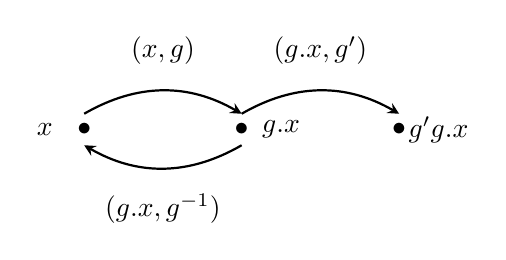
\begin{tikzpicture}
\draw  (0,1) node {$(x,g)$};
\draw  (0,-1) node {$(g.x,g^{-1})$};
\draw  (2,1) node {$(g.x,g')$};
\draw [>=stealth, ->, thick] (-1,0.2) to[bend left] (1,0.2);
\draw [>=stealth, ->,thick] (1,-0.2) to[bend left] (-1,-0.2);
\draw [>=stealth, ->, thick] (1,0.2) to[bend left] (3,0.2);
\draw  (-1,0) node {$\bullet$};
\draw  (-1.5,0) node {$x$};
\draw  (1,0) node {$\bullet$};
\draw  (1.5,0) node {$g.x$};
\draw  (3,0) node {$\bullet$};
\draw  (3.5,0) node {$g'g.x$};
\end{tikzpicture}\]
and this picture gives every element to reconstruct the groupoid.\\

\item[$\bullet$] If $R\subseteq X\times X $ is an equivalence relation, then $R$ as a canonical structure of groupoid with the base space being the diagonal $R^0 = \{ (x,x) \ | \ x\in X\}$ and the multiplication being the only one possible
\[(x,y)(y,z) = (x,z).\] 

\item[$\bullet$] More interesting is the \textit{coarse groupoid} $G(X)$ associated to a discrete countable metric space $(X,d)$ with bounded geometry, that is
\[\sup_{x\in X} |B(x,R)| < \infty \quad \forall R>0.\]
A nice way of thinking about this condition is to imagine yourself looking at the space with a magnifying glass of prescribed radius, but as great as you wish. Then you should not observe more and more points in your sight as you move around. In other words, the points fitting in the radius of your glass is uniformly bounded.\\

Now consider the $R$-diagonals:
\[\Delta_R = \{(x,y) \ | \ d(x,y) < \infty\}\subseteq X\times X\]
and take their closure $\overline{\Delta_R }$ in $\beta (X\times X) $ ($\beta Y$ being the Stone-\v{C}ech compactification of $Y$). The coarse groupoid is defined topologically as 
\[G(X) = \cup_{R>0} \overline{\Delta_R} \rightrightarrows \beta X ,\]
and is endowed with the structure of an \textit{ample} groupoid which extend the groupoid $X\times X \rightrightarrows X$ associated with the coarsest equivalence relation on $X$. The topological property of this groupoid encodes the metric or \textit{coarse} property of the space. For instance, $X$ has property A iff $G(X)$ is amenable, $X$ is coarsely embeddable into a Hilbert space iff $G(X)$ has Haagerup's property, etc.\\
\item[$\bullet$] The last construction is associated to what is often referred as an \textit{approximated group}, which is the data of $\mathcal N = \{ \Gamma , \{N_k\}\}$ where $\Gamma$ is a discrete group, and the $N_k$'s are a tower of finite index normal subgroups with trivial intersection, i.e. 
\[N_1 \triangleleft N_2 \triangleleft ... \quad \text{s.t. } \cap_k N_k = \{ e_\Gamma\} \text{ and } [\Gamma	: N_k] < \infty.  \]
Then the $\Gamma_k$'s are finite groups. Set $\Gamma_\infty = \Gamma$ for convenience (which is not usually finite!). For any discrete group $\Lambda$, there exists a left-invariant proper metric, which is unique up to coarse equivalence (take any word metric if the group is finitely generated). Let us denote by $|\Lambda |$ the coarse class thus obtained. Then the first object of interest in that case is the coarse space $X_\mathcal{N}$ defined as the \textit{coarse disjoint union}
\[X_\mathcal{N} = \coprod_k |\Gamma_k |.\]
Here the metric is such that $d(| \Gamma_i| , |\Gamma_j| )\rightarrow \infty $ as $i+j$ goes to $\infty$, $i\neq j$.\\

The second interesting object attached to $\mathcal{N}$ is the HLS (after Higson-Lafforgue-Skandalis \cite{HLS}, where it was first defined to build counter-examples to the Baum-Connes conjecture) groupoid. The base space is the Alexandrov compactification  of the integers 
\[G_\mathcal{N}^0 = \overline{\N},\]
and $G_\mathcal{N}$ is a bundle of groups with the fiber of $k$ being $\Gamma_k$. The topology is taken to be discrete over the finite base points, and a basis of neighborhood of $(\infty,\gamma)$ is given by 
\[\mathcal{V}_{\gamma, N} = \{(k, q_k(\gamma)) \ | \ k\geq N \} \quad N\in\N ,\]
where $q_k : \Gamma \rightarrow \Gamma_k$ is the quotient map.\\
 \end{itemize}

Problem: Show that a discrete groupoid admits a decomposition of the type 
\[G \cong \coprod_{s\in \Omega} G_s \times (X_s \times X_s)\]

\section{Lecture 14}

If $G$ is a discrete groupoid, and $x\in G^0$, we denote by $G_x$ the group stabilizer of $x$, 
\[G_x = \{g\in G \ : \ s(g)=r(g)=x\}\]
and $X_x$ the orbit of $x$, $X_x = r(s^{-1}(\{x\}))$.\\

Let $\Omega \subset G^0$ be a \textit{fundamental domain}, i.e. $|\Omega \cap X_s| = 1$ for all $s\in \Omega$. Then, if $G_s \times (X_s\times X_s)$ denotes the product of the groupoid $G_s$ (over a point) and the pair groupoid over $X_s$, we have the following result.

\begin{prop}[Green's isomorphism]
There is an isomorphism of groupoids
\[G \cong \coprod_{s\in \Omega} G_s \times (X_s\times X_s).\]
\end{prop}
\begin{proof}
For each $s\in \Omega$ and $x\in X_s$, choose $\gamma_s(x)$ such that $s(\gamma_s(x))=s$ and $r(\gamma_s(x))=x$. Then 
\[\begin{split}
g & \mapsto (\gamma_s(y)^{-1}g\gamma_s(x), (x,y)) \\
(\alpha, (x,y)) & \mapsto \gamma_s(y)\alpha \gamma_s(x)^{-1} \\
\end{split}\]
are groupoid morphisms, and inverse to each other.
\end{proof}

Some examples of groupoids.\\

\textbf{Definition of HLS groupoids} They were defined by Higson-Lafforgue-Skandalis to provide counterexamples to the Baum-Connes conjecture for groupoids. They were used by Willett to provide an example of a non-amenable groupoid such that $C^*_r(G)\cong C^*_m(G)$. \\

\textbf{An important construction} The groupoid of germs of a pseudogroup.

\begin{definition}
Let $X$ be a topological space. A pseudogroup on $X$ is a sub-inverse-semigroup of $Phomeo(X)$, the inverse semigroup of partial homeomorphisms of $X$.
\end{definition}

To a pseudogroup $S$, one can associate the following groupoid $G(S)$.
\begin{itemize}
\item[$\bullet$] As a set, \[G(S) = \{(x,\phi)\in X\times S \ : \ x\in D(\phi)\} / \sim\]
where $(x,\phi)\sim (y,\psi)$ if $x=y$ and there exists a neighborhood $U$ of $x$ such that $\phi_{|U}=\psi_{|U}$. The equivalence class of $(x,\phi)$ is denoted by $[x,\phi]$.
\item[$\bullet$] $s([x,\phi]) = x$ and $r([x,\phi]) = \phi(x)$, $[\phi(x),\psi]\cdot [x,\phi] = [x, \psi\phi]$ where the product of the map is understood in terms of the semigroup operation, $e_x = [x,id_X]$.
\item[$\bullet$] The topology is generated by the sets
\[\mathcal U_{U, \phi} = \{[x,\phi] \ : \ x\in U \}\]
for $\phi\in S$ and $U\subset D(\phi)$ open subset.
\end{itemize} 

Next time: $G(S)$ is \'etale. What is $G(S)$ when $S$ is given by a group action? Also, this gives: the groupoid of an inverse semigroup, the coarse groupoid, the Weyl groupoid of a Cartan pair $(A,B)$.

\section{To do}
Positive type and conditionally negative type functions on groups: the $G$-equivariance gives a unitary (or orthogonal representation), i.e.
\[\phi: G\rightarrow H \iff (H,\pi,v) \text{ GNS triple}.\] 
GNS construction $\phi(g) = \langle v,\pi(g)v\rangle$, i.e. $\phi(s^{-1}t) = \langle \pi(s)v,\pi(t)v\rangle$ which is positive. $\eta(g)= \|\pi(g)v -v\|$. \\

$G$ is a-T-menable (metrically proper action by affine isometries on a real Hilbert space) iff there exists a $G$-equivariant proper negative type function on $G$.\\

Consequence: there is a homotopy between the trivial representation and the regular representation.\\

Gelfand Raikov theorem\\

Do a table with the different definitions and their formulation: historical, kernels and positive functions, Schur multipliers, geometrical, representation theoretical.

\newpage
\section*{Summary}
In the case we look at a group $G$ (top row), and the metric space is $|G|$, then the following holds: 
\[\begin{tikzcd}
\text{(Amenable)} \arrow[r,Rightarrow]\arrow[d,Rightarrow] & \text{(Haagerup)} \arrow[d,Rightarrow]\\
\text{Property (A)} \arrow[r,Rightarrow] & \text{(CEH)} \\
\end{tikzcd}.\]
If $G$ is residually finite, and $X= X_{\mathcal N}(G)$ is the associated box-space, then
\[\begin{tikzcd}
G \text{ is amenable }  \arrow[r,Leftrightarrow]\arrow[dd,Rightarrow] & X \text{ has property (A)} \arrow[d,Rightarrow]\\
	& X \text{ is (CEH)}\arrow[d,Rightarrow] \\
	G \text{ has Haagerup's property }\arrow[ur,Rightarrow]\arrow[r,Leftrightarrow] 	& X \text{ has a fibred (CEH)} \\
\end{tikzcd}.\]
and 
\[\begin{tikzcd}
G \text{ has (T)} \arrow[r,Rightarrow]\arrow[d,Leftrightarrow] & G \text{ has } (\tau)_{\mathcal N}\arrow[d,Leftrightarrow]\\
X_{\mathcal N}(G) \text{ has geometric (T)}\arrow[r,Rightarrow] 	& X_{\mathcal N}(G)\text{ is an expander} \\
\end{tikzcd}.\]
It is still true in general that
\[  X \text{ has } (T)_{geom}\Rightarrow X \text{ is an expander}\]
even if it follows from the previous diagram of implications that a box space of an a-T-menable group with property $(\tau)_{\mathcal N}$ is an expander which does not have geometric (T). $SL(2,\Z)$ with the nested family of congruence subgroups $N_k : ker \ SL(2,\Z) \rightarrow SL(2,\Z / p^k )$ provide such an example.

\begin{table}[h]
\[\begin{array}{|c|c|c|}
\hline
                                                     & \textbf{Amenability} & \textbf{Haagerup}   \\
\hline
\textbf{Geometrical} &  
		\forall \varepsilon, r>0,   & 
		\exists \alpha : G \rightarrow Aff(H)  \\ 
			& \exists F\subset G \text{ finite s.t. }  & \text{ metrically proper} \\
			& \frac{|F\Delta s F|}{|F|}\leq \varepsilon \quad \forall |s|\leq r & \\
\hline
\textbf{Kernels} &
		\forall \varepsilon, r>0, &
		\exists \phi: G\rightarrow \R  \\
			&\exists \phi: G \rightarrow \R \text{ finite support, PT s.t. } & \text{ CNT and proper} \\
			& \|1-\phi\|_{\infty,B_r}\leq \varepsilon  & \\
\hline
\textbf{Hulanicki-Reiter} &
		\forall \varepsilon, r>0, &
		\\
			&\exists f\in l^2(G)_{+,1}\text{ finite support s.t. } & \\
		&  \|s\cdot f -f\|_2< \varepsilon \quad \forall |s|\leq r & \\
\hline
\end{array}\]
\end{table} 

%%%%%%%%%%%%%%%%%%%
\begin{table}[h]
\[\begin{array}{|c|c|c|}
\hline
                                                     &  \textbf{Property (A)}  & \textbf{(CEH)}    \\
\hline
\textbf{Geometrical} &  
		\forall \varepsilon, r>0,   & 
		\exists f: X \rightarrow H   \\ 
			& \exists \{A_x\}_{x\in X}, A_x\subset X\times \mathbb N \text{ finite s.t. } &\text{coarse embedding} \\
			& \frac{|A_x\Delta A_y|}{|A_x\cap A_y|}\leq \varepsilon \quad \forall (x,y)\in \Delta_r & \\
\hline
\textbf{Kernels} &
		\forall \varepsilon, r>0, &
		\exists \phi: X\times X\rightarrow \R \text{ s.t. } \\
			&\exists \phi: X\times X\rightarrow \R \text{ PT s.t. } & \text{ CNT, proper and} \\
			&supp(\phi)\subset \Delta_s \& \|1-\phi\|_{\infty,\Delta_r}\leq \varepsilon  & \text{ bounded on entourages}\\
\hline
\textbf{Higson-Roe} &
		\forall \varepsilon, r>0, &
		\\
			&\exists s>0, f: X\rightarrow  l^2(X)_{+,1}\text{ s.t. } & \\
		&   supp(f(x))\subset \Delta_s \& \|f(x) -f(y)\|_2\leq\varepsilon , \forall (x,y)\leq \Delta_r & \\
\hline
\end{array}\]
\end{table} 
%%%%%%%%%%%%%%%%%%%%

\newpage
\section{Problems}

\subsection{Metric spaces}
Draw the Cayley graphs of $\Z$, $PSL(2,\Z)$, $\Z / (n) \ast \Z / (m)$ and Heisenberg.\\

Use a software to get the first Cayley graphs of $PSL(2,\Z_p)$.\\

Can two non isomorphic groups have isomorphic Cayley graphs? Yes, take two finite groups of same cardinality, and use the whole group minus the identity as a generating subset.\\

\textbf{Milnor Svarc lemma} Show the following result, due to Milnor Svarc.  
\begin{thm}
Let $X$ be a proper geodesic metric space, and $G$ a group which acts on $X$ by isometries. If the action is proper and cocompact, then $G$ is finitely generated and the map
\[G \rightarrow X ; g\mapsto g\cdot x\]
is a quasi-isometry for any $x\in X$.
\end{thm}

\textbf{Isometric embedding into $l^\infty$} Show that all metric spaces are embeddable into a Banach space. 
\[x\mapsto d(x, *)-d(x_0, *), X\rightarrow l^\infty (X)\]

\subsection{Kernels}

Show that \[\phi \left\{\begin{array}{rcl} \R_+ \times \R_+ & \rightarrow & \R \\ (s,t) & \mapsto & \min(s,t)\end{array}\right.\]
is a symmetric positive type kernel on $\R_+$.\\

Let $R\subset X\times X$. Show that $R$ is an equivalence relation iff $\chi_R$ is a symmetric positive type kernel and $\Delta\subset R$.\\
 
Let $f=\sum_n a_n z^n$ be an entire function with $a_n\leq 0$, and let $k: X\times X\rightarrow \R$ be a symmetric positive kernel. Describe the $GNS$-representation associated to $\sum_n a_n k(x,y)^n$ in terms of $GNS(k)$.\\

\textbf{Groups} \\

Let $H<G$ be a subgroup. Show that $\phi(g)=\chi_H(g)= 1_{g\in H}$ defines a positive type function on $G$. Describe its GNS representation. (Hint: start with $H=1$)\\

Give examples of amenable and a-T-menable groups. Give examples of property (A) and (CEH) metric spaces.\\ 

Use the Hulanicki-Reiter condition to prove that
\begin{itemize}
\item[$\bullet$] $\mathbb F_2$ is not amenable.
\item[$\bullet$] amenabilty is invariant by quasi-isometry.	
\end{itemize}

Give a  metrically proper action of $\R^n$ by affine isometries on a real Hilbert space.\\

Show that if a group is acting properly on a tree, then it is a-T-menable.\\

Prove that the left regular representation of a discrete group $G$ cannot have a non-zero invariant vector unless $G$ is finite.\\

\textbf{Universal results} \\

Show that a metric space $(X,d)$ admits an isometric embedding into a Hilbert space iff $\phi(x,y) = d(x,y)^2$ is a symmetric negative type kernel.\\

Show that for any separable Banach space $E$, there exist
\begin{itemize}
\item[$\bullet$] a continuous injective linear map $E\rightarrow l^\infty$,
\item[$\bullet$] a continuous surjective linear map $l^1 \rightarrow E$.   
\end{itemize}
This result shows that $l^1$ and $l^\infty$ are \text{universal}: any Banach space can be realized as a quotient and a subspace of these.

\subsection{Groupoids}

\textbf{Finite quantum mechanical systems} Let $H$ be a self-adjoint matrix. Describe the spectrum of the operator
\[Ad_{H}:\left\{\begin{array}{rcl} M_n(\C) & \rightarrow & M_n(\C) \\ a & \mapsto & [H,a] \end{array}\right.\]
in terms of the spectrum of $H$. Solve the differential equation $a'(t) = [H,a(t)]$.\\

\textbf{First isomorphism theorem} Let $\mathcal I $ be the pair groupoid on $\{0,1\}$. Show that for any groupoid $G$ and any $g\in G$, there exists a unique morphism $\phi: \mathcal I \rightarrow G $ such that $\phi((0,1))=g$. Show that the first isomorphism theorem fails for groupoids. 

\subsection{$C^*$-algebras}

\textbf{Commutation relation} Show that the canonical commutation relation \[ pq-qp = 1\]
does not have a bounded representation. A way to refomulate that is: show that the unital $*$-algebra 
\[ \C^*( p,q | pq-qp =1)\]
does not have any $C^*$-completion. Find a representation of $p$ and $q$ as operators on a Hilbert space, where one of them is allowed to be unbounded. \\

\textbf{Classification of finite dimensional $C^*$-algebras} Let $A$ be a $C^*$-algebra, finite dimensional as a $\C$-vector space. Show there exist positive integers $n,k_1,...,k_n$ and a $*$-isomorphism
\[A\cong \bigoplus_{i=1}^n M_{k_i}(\C).\]

\textbf{Finite groups} Let $G$ be a finte group. Describe the GNS theorem for $A=\C[G]$. Do it for compact groups.\\

\textbf{Commutative groups} How is Pontryagin duality and Gelfand's theorem on commutative $C^*$-algebra related?\\

\textbf{Fell's trick and Green's isomorphism}
First show Fell's trick in a combinatorial manner, i.e. show that the permutation action of $G$ on itself absorb any action of $G$ on a set $X$. Use this to show that 
\[\lambda_G \otimes \pi \cong \lambda_G \otimes 1\]
Same for Green's isomorphism: show that $X\rtimes G \cong \coprod_{s\in \Omega} G_s\times (X_s\times X_s)$ and use it to prove
\[C_0(X)\rtimes_r G \cong \bigoplus_{s\in \Omega} C^*_r(G_s)\otimes \mathfrak K(l^2(X_s)). \]

\textbf{Roe algebras}
Show that 
\[C^*_u(G) \cong l^\infty(G)\rtimes_r G.\]

 
